\newpage
\subsection{The protective battery case}

\begin{figure}[!h]
    \centering
    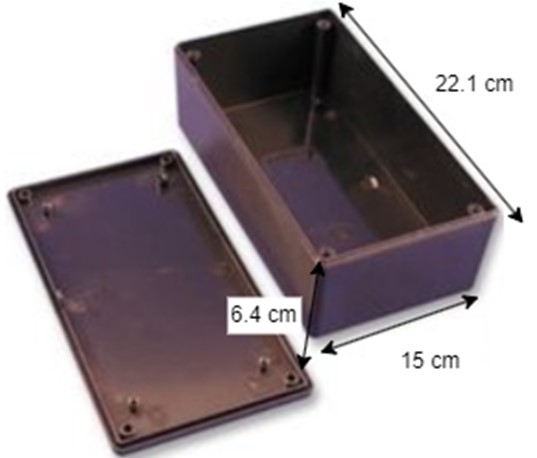
\includegraphics[width=0.8\textwidth]{\currfiledir/figures/case2.jpg}
    \caption{Battery box}
\end{figure}

When exposed to direct sunlight, batteries can overheat and degrade, shortening their lifespan and reducing their efficiency. By placing the battery inside the box, the battery is shielded from the sun's direct heat and is able to maintain a cooler operating temperature.
This protection helps to extend the lifespan of the battery and ensure that it functions optimally in the harsh environmental conditions of the tropical forest.
To protect the battery from direct sunlight and heat, a secondary battery box will be incorporated into the design of the system. This box will be located underneath the main box and will be designed specifically to shield the battery from the sun's direct heat, which can cause the battery to overheat and degrade.
